\section{Motor BLDC}
\label{sec:motor_bldc}

Para fins de resultados pertinentes à equipe Albatroz Aerodesign,designou-se o motor \textit{Scorpion A-5025-310Kv} como unidade sob ensaio. A caracterização do motor exige a identificação experimental de seus parâmetros elétricos e mecânicos, os quais alimentam tanto o modelo dinâmico quanto o observador de estados.

\subsection{Parâmetros Elétricos}
\label{sec:params_eletricos}

Para a determinação da resistência e da indutância de fase, emprega-se o ensaio de rotor bloqueado, cujo circuito equivalente está ilustrado na Figura \ref{fig:circuito_estrela_bldc}. O travamento mecânico do eixo impede a indução de forças contraeletromotrizes decorrentes de micro-oscilações, reduzindo o modelo elétrico do motor a uma malha puramente passiva em ligação estrela\footnote{Este equacionamento é válido independentemente do fechamento interno real da máquina. Para um motor fechado em delta, a impedância medida linha a linha equivale a duas fases em série em paralelo com a terceira ($Z_{linha} = \frac{2}{3}Z_{\Delta}$). Como a transformação para o modelo equivalente em estrela requer $Z_Y = \frac{Z_{\Delta}}{3}$, chega-se à mesma relação final $Z_Y = \frac{Z_{linha}}{2}$, permitindo modelar o motor a partir dos terminais como uma caixa preta.}.

\begin{figure}[H]
    \centering
    \caption{Circuito Equivalente do Motor BLDC (Rotor Bloqueado) }

    \begin{tikzpicture}[transform shape, american]
        % Ponto Neutro
        \node[circ] (N) at (0,0) {};
        \node[above left, xshift=-0.1cm] at (N) {$N$};

        % Fase U (Para Cima)
        \draw (N) to[american resistor, l=$R_{fase}$] (0,2)
                  to[cute inductor, l=$L_{fase}$] (0,4)
                  node[ocirc] (U) {}
                  node[above] {Fase $U$};

        % Fase V (Para a Direita/Baixo) - Ângulo de -30°
        \draw (N) to[american resistor, l=$R_{fase}$] (1.732,-1)
                  to[cute inductor, l=$L_{fase}$] (3.464,-2)
                  node[ocirc] (V) {}
                  node[right] {Fase $V$};

        % Fase W (Para a Esquerda/Baixo) - Ângulo de 210°
        \draw (N) to[american resistor, l_=$R_{fase}$] (-1.732,-1)
                  to[cute inductor, l_=$L_{fase}$] (-3.464,-2)
                  node[ocirc] (W) {}
                  node[left] {Fase $W$};

        % --- Indicação do Ensaio (Medição Linha a Linha) ---

        % Linhas de chamada (tracejadas) saindo de U e V para a direita
        \draw[dashed, blue!70!black] (U) -- (5.5, 4);
        \draw[dashed, blue!70!black] (V) -- (5.5, -2);

        % Seta dupla indicando a medição com texto explicativo
        \draw[<->, blue!70!black, thick] (5.5, 3.9) -- node[fill=white, align=center, text=black] {Ensaio Linha a Linha \\ $V_{DC}, I_{DC}$ (Resistência) \\ $L_{linha}$ (Indutância) \\ \small \textit{Equivalente a 2 em série}} (5.5, -1.9);

        % Marcação do caminho da corrente para ficar mais didático (Opcional)
        \draw[->, red, thick, rounded corners=5mm] (0.5, 3.5) -- (0.5, 0.5) -- (3.0, -1.0) node[pos=0.8, above right] {$I_{ensaio}$};

    \end{tikzpicture}
    \label{fig:circuito_estrela_bldc}

    \small Fonte: Autor (2026)
\end{figure}

A resistência de fase é medida aplicando-se uma corrente contínua entre dois terminais do motor. Nesta condição, a reatância indutiva é nula e a queda de tensão ocorre integralmente sobre as resistências. Medindo-se a tensão ($V_{DC}$) e a corrente ($I_{DC}$), a resistência de fase equivalente é calculada por:

\begin{equation}
    R_{fase} = \frac{V_{DC}}{2\,I_{DC}}
    \label{eq:resistencia_fase}
\end{equation}


De maneira análoga, com o rotor ainda imobilizado, conduz-se o ensaio para a
obtenção da indutância de fase através do método da ressonância. Motores BLDC
aplicados em aeromodelismo, como o \textit{Scorpion A-5025}, geralmente possuem
ímãs montados na superfície do rotor (SPM --- \textit{Surface Permanent
Magnet}). O entreferro efetivamente uniforme característico dessa topologia
torna a saliência magnética insignificante, permitindo assumir que as
indutâncias de eixo direto ($L_d$) e em quadratura ($L_q$) são aproximadamente
iguais ($L_d \approx L_q \approx L_s$), onde $L_s$ é a indutância síncrona da
máquina \cite{Krishnan2017}.

Na ausência de um medidor LCR, o ensaio consiste em associar um capacitor de
valor conhecido ($C$) em paralelo com o enrolamento da máquina, formando um
circuito ressonante $LC$ alimentado por uma fonte senoidal de frequência
variável através de um resistor série $R$, conforme a
Figura~\ref{fig:circuito_ressonancia_v2}. Ao varrer a frequência da fonte até
atingir a frequência de ressonância ($f_r$), na qual a impedância do tanque
$LC$ é máxima e a tensão sobre ele atinge seu valor de pico, a indutância pode
ser estimada \cite{Fitzgerald2014}. A condição de ressonância corresponde ao
ponto em que a reatância do circuito se anula, restando apenas as componentes
resistivas. Após determinar a indutância equivalente medida entre dois
terminais ($L_{linha}$), a indutância de fase individual é obtida pela relação
de ressonância:

\begin{figure}[htbp]
    \centering
    \caption{Circuito de ensaio de ressonância: resistor $R$ em série com o
    paralelo $L$--$C$, com a tensão de ressonância medida sobre o tanque.}
    \label{fig:circuito_ressonancia_v2}
    \begin{circuitikz}[american, scale=1.1, transform shape]
        % ---- Fonte e resistor série (ramo superior) ----
        \draw (0,0) to[sV, l=$v_{in}$] (0,3);
        \draw (0,3) to[R, l=$R$, i>^=$i_{in}$] (3,3);
        % ---- Nó de medição (saída do gerador / topo do tanque) ----
        \node[circ] (A) at (3,3) {};
        \node[anchor=south] at (3,3.2) {\footnotesize nó A};
        % ---- Ramo do indutor ----
        \draw (A) to[L, l=$L_{fase}$] (3,0);
        % ---- Ramo do capacitor (em paralelo) ----
        \draw (A) -- (5.5,3);
        \draw (5.5,3) to[C, l=$C$] (5.5,0);
        % ---- Trilho de terra (retorno) ----
        \draw (0,0) -- (5.5,0);
        \node[circ] (G) at (3,0) {};
        \node[ground] at (1.5,0) {};
    \end{circuitikz}

    \fonte{Autor (2026).}
\end{figure}

\begin{equation}
    f_r = \frac{1}{2\pi\sqrt{L_{linha} \cdot C}}
    \implies
    L_{linha} = \frac{1}{C\,(2\pi f_r)^2}
    \label{eq:ressonancia_L}
\end{equation}

Considerando a topologia de conexão dos enrolamentos, a indutância de fase
individual é dada por:

\begin{equation}
    L_{fase} = \frac{L_{linha}}{2}
    \label{eq:indutancia_fase}
\end{equation}

Este valor de $L_{fase}$ é diretamente empregado como o parâmetro $L_s$ nas
equações de espaço de estados no referencial estacionário $\alpha\beta$.

\subsection{Parâmetros Mecânicos}
\label{sec:params_mecanicos}

A dinâmica mecânica do motor é governada pela equação de balanço de torques no eixo rotativo, como visto na \autoref{eq:bldc_mecanica}.

Os ensaios de atrito e de inércia descritos nesta subseção foram conduzidos
sem a hélice acoplada ao eixo, de modo que $B$, $\tau_c$ e $J$ correspondem
exclusivamente ao conjunto girante do próprio motor (rotor, eixo e
rolamentos). Com a hélice montada para os ensaios aerodinâmicos
(\autoref{sec:coef_aero_bancada}), o diâmetro e o passo do modelo utilizado
propagam-se para $D_{prop}$ nas Equações~\eqref{eq:Prop_coeff1} e
\eqref{eq:Prop_coeff2}, conforme a nomenclatura $D \times P$ da
\autoref{sec:helice_aerodinamica}.

Para a caracterização experimental, o motor BLDC é acionado utilizando um Controlador Eletrônico de Velocidade (ESC) comercial. Como o torque eletromagnético ($T_e$) em motores de ímã permanente é proporcional à corrente de eixo em quadratura ($I_q$), a bancada de testes irá ser instrumentada para adquirir as correntes instantâneas de fase do motor. O esquema de \textit{hardware} e as formas de onda esperadas estão ilustrados na Figura \ref{fig:circuito_esc_correntes}.

\begin{figure}[H]
    \centering
    \caption{Esquema de Medição com ESC e Transformação de Correntes ($abc \to dq$)}

    % --- PARTE 1: CIRCUITO DE \textit{hardware} COM AJUSTES DE LEGENDA ---
    \begin{tikzpicture}[auto, node distance=2cm, >=latex']

        % --- Blocos principais ---
        \node [draw, rectangle, minimum height=3em, minimum width=4em] (bat) {Bateria};

        % Aumentei para 8em para comportar o deslocamento das fases com folga
        \node [draw, rectangle, minimum height=8em, minimum width=4em, right=of bat, node distance=2.5cm] (esc) {ESC};

        % BLDC posicionado à direita
        \node [draw, rectangle, rounded corners=8pt, minimum height=8em, minimum width=5em, right=of esc, node distance=6.5cm] (motor) {BLDC};

        % SAME/DAQ centralizado abaixo
        \node [draw, rectangle, minimum height=4em, minimum width=10em, below=of esc, node distance=4.5cm, xshift=3.25cm] (daq) {SAME / DAQ};

        % --- Conexões Bateria -> ESC ---
        \draw [thick] ([yshift=0.3cm]bat.east) -- node[above] {$V_{DC}$} ([yshift=0.3cm]esc.west);
        \draw [thick] ([yshift=-0.3cm]bat.east) -- node[below] {GND} ([yshift=-0.3cm]esc.west);

        % --- Coordenadas das Fases (A, B, C) ---
        % Deslocadas para cima (+0.5cm) para não bater no centro (0) do Eixo
        \coordinate (esc_a) at ([yshift=1.5cm]esc.east);
        \coordinate (esc_b) at ([yshift=0.5cm]esc.east);
        \coordinate (esc_c) at ([yshift=-0.5cm]esc.east);

        \coordinate (mot_a) at ([yshift=1.5cm]motor.west);
        \coordinate (mot_b) at ([yshift=0.5cm]motor.west);
        \coordinate (mot_c) at ([yshift=-0.5cm]motor.west);

        % --- Conexões das Fases ---
        \draw [thick] (esc_a) -- node[above, pos=0.5, font=\large\bfseries] {A} (mot_a);
        \draw [thick] (esc_b) -- node[above, pos=0.5, font=\large\bfseries] {B} (mot_b);
        \draw [thick] (esc_c) -- node[below, pos=0.5, font=\large\bfseries] {C} (mot_c);

        % --- Sensores de Corrente (Intercalados) ---
        % Sensor A (Violeta) próximo ao ESC
        \node [draw, circle, minimum size=0.45cm, inner sep=0pt, thick, fill=white] (sensA) at ([xshift=1.2cm]esc_a) {};
        % Sensor B (Teal) próximo ao Motor
        \node [draw, circle, minimum size=0.45cm, inner sep=0pt, thick, fill=white] (sensB) at ([xshift=1.5cm]esc_b) {};

        % --- Sensor de Posição Óptico (No Eixo Central) ---
        \node [draw, rectangle, minimum height=2em, right=of motor, node distance=2.2cm] (enc) {Sensor};
        % O Eixo sai do centro exato (0), onde agora não há fios
        \draw [thick, dashed] (motor.east) -- node[above] {Eixo} (enc.west);

        % --- Conexões de Dados para o SAME (Intercaladas) ---
        % Sensor A desce mais (3.5cm)
        \draw [->, dashed, violet, thick] (sensA.south) -- ++(0,-3.5) -| ([xshift=-1.2cm]daq.north);

        % Sensor B desce menos (1.8cm)
        \draw [->, dashed, teal, thick] (sensB.south) -- ++(0,-3.5) -| ([xshift=-0.9cm]daq.north);

        % Sensor de posição vem pela lateral
        \draw [->, dashed, thick] (enc.south) |- (daq.east) node[pos=0.8, above] {$\theta, \omega$};

        % --- Label de transformação ---
        \node [below, font=\scriptsize, text width=5cm, align=center] at (daq.south) { $I_c = -(I_a + I_b)$ \\ Clarke \& Park $\to I_d, I_q$};

    \end{tikzpicture}

    \vspace{0.8cm} % Espaço entre o circuito e os gráficos

    % --- PARTE 2: GRÁFICOS DAS CORRENTES COM AJUSTES DE EIXO ---
    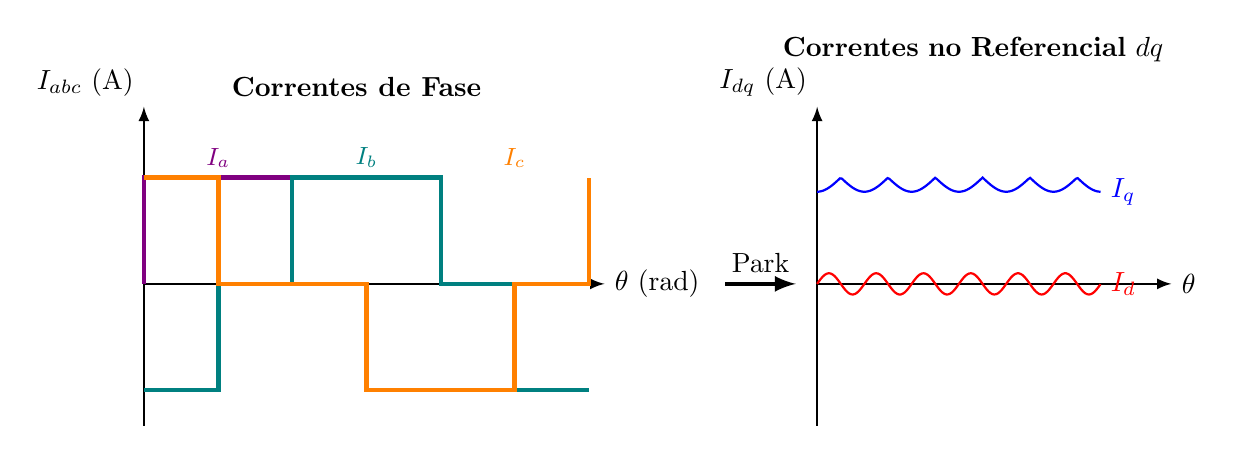
\begin{tikzpicture}[scale=0.9, >=latex]

        \begin{scope}[xshift=0cm]
            \draw[->, thick] (0,-2) -- (0,2.5) node[above left] {$I_{abc}$ (A)};
            \draw[->, thick] (0,0) -- (6.5,0) node[right] {$\theta$ (rad)};

            % Curva Ia (120 graus ligada, 60 desligada)
            \draw[ultra thick, violet] (0,0) -- (0,1.5) -- (2.09,1.5) -- (2.09,0) -- (3.14,0) -- (3.14,-1.5) -- (5.23,-1.5) -- (5.23,0) -- (6.28,0);
            \node[above, violet, font=\small\bfseries] at (1.05, 1.5) {$I_a$};

            % Curva Ib (Atrasada 120 graus)
            \draw[ultra thick, teal] (0,-1.5) -- (1.05,-1.5) -- (1.05,0) -- (2.09,0) -- (2.09,1.5) -- (4.19,1.5) -- (4.19,0) -- (5.23,0) -- (5.23,-1.5) -- (6.28,-1.5);
            \node[above, teal, font=\small\bfseries] at (3.14, 1.5) {$I_b$};

            % Curva Ic (Adiantada 120 graus)
            \draw[ultra thick, orange] (0,1.5) -- (1.05,1.5) -- (1.05,0) -- (3.14,0) -- (3.14,-1.5) -- (5.23,-1.5) -- (5.23,0) -- (6.28,0) -- (6.28,1.5);
            \node[above, orange, font=\small\bfseries] at (5.23, 1.5) {$I_c$};

            \node[above] at (3, 2.5) {\textbf{Correntes de Fase}};
        \end{scope}

        % --- Seta de Transformação ---
        \draw[->, ultra thick] (8.2, 0) -- node[above, black] {Park} (9.2, 0);

        % --- Gráfico 2: Correntes FOC (dq) com RIPPLE ---
        \begin{scope}[xshift=9.5cm]
            \draw[->, thick] (0,-2) -- (0,2.5) node[above left] {$I_{dq}$ (A)};
            \draw[->, thick] (0,0) -- (5,0) node[right] {$\theta$};

            % Curva Iq (Com ripple de comutação - 6 pulsos)
            \draw[thick, blue, domain=0:4, samples=150] plot (\x, {1.5 - 0.2*abs(cos(4.71*\x r))}) node[right] {$I_q$};

            % Curva Id (Oscilando em torno de zero)
            \draw[thick, red, domain=0:4, samples=150] plot (\x, {0.15*sin(9.42*\x r)}) node[right] {$I_d$};

            \node[above, text width=5cm, align=center] at (2.2, 3) {\textbf{Correntes no Referencial $dq$}};
        \end{scope}

    \end{tikzpicture}

    \label{fig:circuito_esc_correntes}
    \small Fonte: Autor (2026)
\end{figure}

Através do Sistema de Aquisição do Motor Elétrico (SAME), lê-se as correntes de pelo menos duas fases (ex: $I_a$ e $I_b$). Considerando que não há conexão de neutro, a terceira corrente é obtida por $I_c = -(I_a + I_b)$. Sincronizando essas leituras com a posição angular elétrica do rotor ($\theta_e$) --- obtida indiretamente pela medição do sensor óptico --- aplica-se as transformadas de Clarke e Park (\textit{offline} ou \textit{online}) para mapear as grandezas do referencial trifásico estacionário ($abc$) para o referencial síncrono girante ($dq$) \footnote{Devido à natureza da comutação trapezoidal (6-step) do ESC utilizado, as correntes de fase apresentam harmônicos que resultam em oscilações (\textit{ripple}) nas componentes $I_d$ e $I_q$ após a transformada de Park. Para os cálculos de caracterização, utiliza-se o valor médio filtrado de $I_q$, que representa a componente fundamental do torque eletromagnético médio em regime permanente.}.

Os ensaios de atrito e de inércia descritos a seguir foram conduzidos numa
montagem provisória, antes da fabricação e validação das placas definitivas
(SIBA e SAME): o motor é acionado por um ESC comercial, com a rotação do
eixo e as grandezas elétricas de fase medidas de forma independente do
acionamento.

\subsubsection{Coeficiente de Atrito Viscoso}
\label{sec:atrito_viscoso}

Para extrair os coeficientes de atrito ($B$ e $\tau_c$) \footnote{O atrito de Coulomb ($\tau_c$) representa uma parcela de torque constante necessária para vencer a fricção estática e cinética dos rolamentos}, estabiliza-se a rotação do motor a vazio em múltiplos patamares. Em regime permanente ($\frac{d\omega_m}{dt} = 0$), o torque eletromagnético anula exatamente as perdas mecânicas:

\begin{equation}
    T_{e,k}= B\omega_{m,k} + \tau_c
    \label{eq:ensaio_vazio_iq}
\end{equation}

Os parâmetros $B$ e $\tau_c$ são obtidos através de uma regressão linear sobre os pontos experimentais médios $(\omega_{m,k}, T_{e,k})$ para cada patamar de rotação, o $\omega_{m,k}$ é medido através de um tacômetro digital para validação.

\subsubsection{Momento de Inércia}
\label{sec:momento_inercia}

Com o atrito estabelecido, o momento de inércia ($J$) é estimado pelo ensaio de desaceleração livre (\textit{coast-down}). Ao atingir a rotação nominal máxima, a aceleração via ESC é cortada. Sem excitação externa, as correntes caem a zero ($I_q = 0$), zerando o torque motriz. A dinâmica de parada é descrita por:

\begin{equation}
    J \frac{d\omega_m}{dt} = - B\omega_m - \tau_c
    \label{eq:coast_down_iq}
\end{equation}

O sensor óptico registra a curva de desaceleração $\omega_m(t)$. Isolando $J$ e calculando a derivada $\frac{d\omega_m}{dt}$ a partir dos dados adquiridos na região de decaimento, extrai-se o momento de inércia do conjunto rotativo.

\subsection{Identificação dos Coeficientes Aerodinâmicos da Hélice em Bancada}
\label{sec:coef_aero_bancada}

Com a hélice já montada no eixo, o motor é levado por patamares de
aceleração crescente, do menor ponto em que ele ainda gira de forma estável
até a rotação máxima permitida. A \autoref{fig:fluxo_ensaio_helice} resume
o ensaio: em cada patamar, o motor permanece tempo suficiente para
estabilizar a rotação, seguindo o critério de regime permanente
formalizado no \autoref{alg:kq_identificacao}; só então são registrados a rotação, a
tração medida pela célula de carga, o torque estimado pelo observador e a
densidade do ar, calculada pela \autoref{eq:densidade_calculo} a partir da
pressão e da temperatura do ambiente.

\begin{figure}[H]
    \centering
    \caption{Fluxo do ensaio de identificação dos coeficientes da hélice}
    \label{fig:fluxo_ensaio_helice}
    \begin{tikzpicture}[
        font=\small,
        box/.style={draw, rounded corners, align=center, minimum height=1cm, minimum width=3.1cm, text width=2.9cm},
        arrow/.style={-{Latex}, thick}
    ]
        \node[box] (duty)  at (0,0)   {Novo patamar\\de aceleração};
        \node[box] (estab) at (3.6,0) {Aguarda\\estabilizar};
        \node[box] (reg)   at (7.2,0) {Registra rotação,\\tração e torque};
        \node[box] (calc)  at (10.8,0){Calcula $C_T$ e\\$C_Q$ do patamar};

        \draw[arrow] (duty) -- (estab);
        \draw[arrow] (estab) -- (reg);
        \draw[arrow] (reg) -- (calc);
        \draw[arrow] (calc.north) to[out=60, in=120, looseness=0.5] node[above, font=\scriptsize]{próximo patamar} (duty.north);
    \end{tikzpicture}

    Fonte: Autor (2026)
\end{figure}

O \autoref{alg:kq_identificacao} formaliza o critério de patamar usado
nesse ensaio: a detecção automática dos intervalos de regime permanente a
partir do perfil de referência e o cálculo do coeficiente por patamar.

\begin{algorithm}[H]
\caption{Identificação do coeficiente aerodinâmico global $k_Q$ por patamar}
\label{alg:kq_identificacao}
\begin{algorithmic}[1]
\Require $\omega_m,\hat{\omega}_e,T_e,\hat{T}_e$ (vetores), $R$ (perfil de RPM), $T_s$, $\tau_{\mathrm{PI}}$, $\mathrm{RPM}_{\min}$
\Function{DetectaPatamares}{$R$}
    \State $M \gets (\Delta R = 0) \wedge (R > \mathrm{RPM}_{\min})$
    \State $P \gets$ pares $(s,e)$ dos blocos contínuos de $M$
    \State \Return $P$
\EndFunction
\Statex
\Function{CalculaKQ}{$\omega_m,\hat{\omega}_e,T_e,\hat{T}_e,P$}
    \State $n \gets \tau_{\mathrm{PI}}/T_s$
    \ForAll{$(s,e) \in P$}
        \If{$e-s \le n$}
        \State \textbf{continue}
        \EndIf
        \State $i,j \gets s+n,\ e-1$
        \State $k_1 \gets \overline{T_e[i:j]} \,/\, \overline{\omega_m[i:j]}^{\,2}$
        \State $k_2 \gets \overline{\hat{T}_e[i:j]} \,/\, \overline{\hat{\omega}_e[i:j]}^{\,2}$
        \State guarda $(k_1,k_2)$ em $K$
    \EndFor
    \State $\bar{k}_1,\bar{k}_2 \gets$ médias de $K$
    \State $\epsilon \gets 100\,|\bar{k}_2-k_{Q,\mathrm{nom}}|/k_{Q,\mathrm{nom}}$
    \State \Return $K,\ \bar{k}_1,\ \bar{k}_2,\ \epsilon$
\EndFunction
\end{algorithmic}
\end{algorithm}

Como o ensaio é feito parado, sem vento incidente sobre a hélice
($V_\infty \approx 0$), os coeficientes de tração ($C_T$) e de torque
($C_Q$) de cada patamar são calculados diretamente pelas
Equações~\eqref{eq:Prop_coeff2} e \eqref{eq:Prop_coeff1}.

A referência de comparação são as tabelas de desempenho publicadas pelo
próprio fabricante da hélice (APC) \cite{apc_performance_data}, que
fornecem $C_T$ e $C_P$ em função da razão de avanço $J$ e já incluem a
condição parada, convertendo-se $C_P$ para $C_Q$ pela
\autoref{eq:cq_from_cp}. O banco de dados de hélices da
\textit{University of Illinois Urbana-Champaign} (UIUC) entra como segunda
referência, para hélices da categoria \textit{Thin Electric} equivalentes
\cite{SeligPropDB}.

Como o comportamento aerodinâmico da hélice muda com a rotação (efeito do
número de Reynolds), os coeficientes são reportados por patamar de rotação,
e não como um valor único para toda a faixa de operação.

\subsection{Parametrização do SMO}
\label{sec:param_smo}

Com os parâmetros intrínsecos do motor obtidos, resta o problema de selecionar os ganhos deslizantes ($K_{s1}$, $K_{s2}$) e o polo do estimador ($K_t$). Esses parâmetros condicionam características antagônicas: ganhos elevados aceleram a convergência do erro de predição de corrente, porém amplificam o conteúdo harmônico injetado na BEMF; o polo $K_t$ atenua esse ruído ao custo de atraso de fase dependente da frequência elétrica. Como a frequência elétrica varia ao longo do envelope de operação, não há um conjunto de ganhos trivialmente ótimo, e o ajuste manual revela-se laborioso e pouco reprodutível. Esses fatores motivaram a adoção de um procedimento de ajuste automático \textit{(autotuning)} \textit{offline}, capaz de ser
reaplicado sistematicamente a diferentes conjuntos motopropulsores --- requisito
central para uma bancada de caracterização que se pretende geral.

O procedimento é conduzido sobre a planta computacional do conjunto
motopropulsor, que fornece as referências de torque e velocidade. Ao longo desta seção, essas grandezas geradas pela planta simulada são designadas ``reais'', em contraposição às estimativas produzidas pelo observador; não se trata, portanto, de medições experimentais, mas da referência sintética contra a qual o estimador é ajustado.

O objetivo físico do observador, neste contexto, é estimar com fidelidade as
grandezas de saída do conjunto: o torque de eixo e a velocidade angular. São
essas as variáveis posteriormente empregadas na identificação dos coeficientes
aerodinâmicos. Por essa razão, ao invés de penalizar grandezas internas do
estimador --- como o erro angular, que o PLL já torna pouco discriminante ---, a
função-custo foi formulada como o \textit{seguimento} direto do torque e da
velocidade \cite{hermuche2023funcoes, datacamp2025cost}, mantendo o procedimento
agnóstico aos detalhes internos do observador e, portanto, transferível a outros
motores.

A avaliação ocorre sobre os trechos em regime permanente de cada patamar de
velocidade. Para um patamar $q$, a \autoref{eq:termos_seguimento} define o erro
de seguimento de torque ($g_{T,q}$), a partir das amostras de torque real
($\Tau_{q,n}$) e estimado ($\hat{\Tau}_{q,n}$), e o erro relativo de velocidade
($g_{\omega,q}$), das velocidades médias real ($\varpi_q$) e estimada
($\hat{\varpi}_q$). O termo de torque emprega a função de perda de Huber
($\ell_\delta$), que combina sensibilidade quadrática próxima ao acerto com
robustez linear aos desvios grandes, atenuando o impacto das quedas periódicas
de observabilidade do SMO durante as comutações do inversor sem descartá-las por
completo:
%
\begin{equation}
    g_{T,q} = \frac{1}{N_q}\sum_{n=1}^{N_q}
        \ell_\delta\!\big( \hat{\Tau}_{q,n} - \Tau_{q,n} \big),
    \qquad
    g_{\omega,q} = \frac{\big|\, \hat{\varpi}_q - \varpi_q \,\big|}{|\varpi_q|},
    \label{eq:termos_seguimento}
\end{equation}
%
onde $N_q$ é o número de amostras do patamar e $\ell_\delta(r) = \tfrac{1}{2}r^2$
para $|r|\le\delta$ e $\ell_\delta(r) = \delta\,(|r|-\tfrac{1}{2}\delta)$ caso
contrário. A função-custo agregada, apresentada na
\autoref{eq:custo_autotuning}, é a média ponderada desses erros sobre os $M$
patamares avaliados:
%
\begin{equation}
    J(\mathbf{x}) = \frac{1}{M}\sum_{q=1}^{M}
        \Big( w_T\,g_{T,q} + w_\omega\,g_{\omega,q}\Big),
    \label{eq:custo_autotuning}
\end{equation}
%
com pesos $w_T = \num{1,0}$ e $w_\omega = \num{0,5}$, priorizando deliberadamente
a fidelidade do torque, grandeza de maior interesse para a caracterização
propulsiva. Cabe ressaltar que o valor numérico de $J$ não constitui uma medida
de exatidão global do estimador: a topologia é fortemente não linear e o erro
varia entre patamares, de modo que $J$ deve ser entendido apenas como o índice
relativo que orienta a busca, e não como um erro percentual absoluto.

Na discretização por Euler progressivo, os ganhos atuam sobre a dinâmica do
observador na forma dos produtos definidos na
\autoref{eq:discretizacao_coeff_smo}, de modo que um mesmo comportamento
dinâmico corresponde a valores de $K$ inversamente proporcionais a $T_s$.
Otimizar $K$ diretamente atrelaria o resultado ao passo específico da simulação,
comprometendo sua transferência ao \textit{firmware}, cujo período de execução é
ditado pelo hardware de aquisição. Por essa razão, a otimização é conduzida
sobre os ganhos discretizados $\Gamma$, invariantes ao passo, recuperando-se o
ganho efetivamente embarcado por $K = \Gamma / T_s$ com o $T_s$ real da malha de
controle.

Para condicionar a busca, os parâmetros são otimizados em espaço logarítmico com
sinais fixos, escrevendo $\Gamma=(+1,-1,+1)\odot 10^{\mathbf{x}}$, o que
normaliza as três ordens de grandeza distintas e impõe por construção as
restrições de sinal $\Gamma_{s1}>0$, $\Gamma_{s2}<0$ e $\Gamma_{t}>0$. A
minimização emprega o algoritmo de Evolução Diferencial
(\autoref{alg:autotuning}), executando a simulação em um horizonte reduzido que
cobre os patamares mais exigentes.

\begin{algorithm}[H]
\caption{Ajuste automático de ganhos (offline)}
\label{alg:autotuning}
\begin{algorithmic}[1]
\Require ponto inicial $\mathbf{x}_0$, limites $\mathcal{B}$, perfil reduzido
\Function{Custo}{$\mathbf{x}$}
    \State $\Gamma \gets (+1,-1,+1)\odot 10^{\mathbf{x}}$
    \State $(K_{s1},K_{s2},K_t) \gets \Gamma / T_s$
    \State $\textbf{out} \gets$ \Call{Simular}{$K_{s1},K_{s2},K_t$}
    \If{$\textbf{out}$ não é finito} \State \Return penalidade elevada \EndIf
    \State \Return $J(\textbf{out})$ \Comment{Eq.~\eqref{eq:custo_autotuning}}
\EndFunction
\State $\mathbf{x}^{\star} \gets \displaystyle\operatorname*{arg\,min}_{\mathbf{x}\in\mathcal{B}}\ \textsc{Custo}(\mathbf{x})$
    \Comment{Evolução Diferencial}
\State \Return $\Gamma^{\star} = (+1,-1,+1)\odot 10^{\mathbf{x}^{\star}}$
\end{algorithmic}
\end{algorithm}

A natureza não-convexa de $J$, decorrente do \textit{chattering} e das saturações
da planta, justifica a adoção de um método de otimização livre de gradiente. Os
ganhos resultantes e a verificação de invariância ao passo são reportados na
\autoref{sec:autotuning}.
